\newpage
\graphicspath{{../suyluancungbi/xuanphong/}}
\begingroup
\AddToShipoutPicture*{\put(54,585){
\includegraphics[scale=0.9]{../xuanphong/xuanphong.pdf}}} % %Image background
\centering
\endgroup
\vspace*{50pt}
%	
%	STT	Số/năm	Tên bài	Trang
%	2	08/2019	Thổ ngữ Châu Phi     xxx	9
%	3	03/2020	Du hành trên đại dương    xxxx	46
%	4	05/2020	Thử thách sống còn    xxx	58
%	5	10/2020	Chiếc mũ kỷ niệm  xxx	16
%	6	11/2020	Ba chiếc hộp và cô thư ký   xxx	23
%	8	05/2021	Vị thám tử ẩn danh	xxxx	26
%	
%	
%	Đặt lại  tiêu đề:  …………. ).
%	Tác giả : GIA DƯƠNG
	Một chiều những ngày cuối năm, phóng viên tạp chí Pi có cuộc gặp gỡ ngắn với thanh tra Lê Kính tại văn phong thám tử Xuân Phong.
	\vskip 0.1cm
	PV: Cảm ơn thanh tra đã nhận lời tạp chí. Các độc giả nhỏ tuổi rất mong chờ cuộc gặp gỡ này.
	\vskip 0.1cm
	LK: Tôi rất vui có dịp giao lưu với các bạn nhỏ của Pi. Xuân Phong không thể tham dự vì một việc khẩn cấp, anh ấy đã đi từ sáng sớm.
	\vskip 0.1cm
	PV: Anh có thể kể đôi chút về mình không?
	\vskip 0.1cm
	LK: À, cũng không có gì đặc biệt. Tôi vốn là một bác sỹ nhưng một tai nạn xảy ra đã khiến tôi không tiếp tục công việcnày. Và một sự tình cờ, tôi đã gặp Xuân Phong rồi  cộng tác cùng anh ấy. 
	\vskip 0.1cm
	PV: Anh có thể kể một chút về lần gặp Xuân Phong không?
	\vskip 0.1cm
	LK: Câu chuyện cũng hơi dài dòng nhưng chúng tôi cảm thấy như đã là bạn bè của nhau từ rất lâu rồi.
	\vskip 0.1cm
	PV: Thời gian vừa qua,  các bạn nhỏ rất ngưỡng mộ tài phá án tài tình của các anh. Anh có thể kể cho các bạn nhỏ một vài vụ án được không?
	\vskip 0.1cm
	LK: Ah, tôi  nghĩ là có một số vụ án hợp với các bạn đọc nhỏ tuổi của báo mình đấy, ngoài ra cũng có  vài truyện bên lề  thú vị nữa đấy. (Cười). Tuy nhiên tôi cho là các bạn nhỏ của Pi chắc thích tự khám phá hơn. Thế nên, tôi sẽ kể một vài câu chuyện xảy ra trong lúc thực thi công vụ của chúng tôi thời gian vừa qua, phần còn lại chờ các thám tử nhí “phá án” nhé.
	\vskip 0.1cm
	PV: Tuyệt quá! Xin mời anh Kính.
	\vskip 0.1cm
	Chiều cuối năm, phố xá đã rộn ràng đón tết, thanh tra Lê Kính đưa mắt xa xăm…
	Tôi nhớ như in hai lần đi công tác nước ngoài.
	\vskip 0.1cm
	\newpage
	\textbf{\color{toancuabi}{THỔ NGỮ CHÂU PHI} } %textbf
	\vskip 0.1cm 
	Chúng tôi trải qua mấy lần đổi máy bay ở sân bay Miến Điện rồi Rô--ma Ý -- đại lợi phồn hoa nhưng nực nội, cuối cùng, chúng tôi cũng đáp xuống vùng đất hoang sơ của những cánh rừng bạt ngàn xanh mướt và những đôgnf cỏ trải ngút tận chân trời. 
	\vskip 0.1cm
	-- Đẹp quá phải không anh Phong? Anh xem nơi đây giống thiên đường không. Mai tôi sẽ đưa anh ra chợ của người bản xứ để biết thêm về cuộc sống muôn màu sắc của họ. 
	\vskip 0.1cm
	Sáng hôm sau, tôi dẫn hai con ngựa tới rủ thám tử Phong xuống khu ở của người bản địa thuộc một bộ lạc. Đường đi xuống thung lũng thoai thoải đi qua những dải chuối rừng tựa ở quê nhà, những ruộng ngô tươi tốt sắp tới kì thu hoạch. Tới khu chợ rồi. Chao ơi, mới có vài ngày dùng đồ khô ăn liền, có nấu nướng cẩn thận , nên từ xa mùi thức ăn thơm ngon thật quyến rũ lạ thường.
	\vskip 0.1cm
	-- Anh Kính thử vào đây này. Họ có món gì ngon lắm.
		\vskip 0.1cm
Nghe Xuân Phong gọi, tôi ghé vào quán, phải thử một chút xem hương vị Phi Châu có khác vị Hà Thành không.
	\vskip 0.1cm
	Người đàn ông bán hàng trông thật hóm hỉnh, độc một chiếc khố quấn ngang lưng. Vừa thấy Xuân Phong nhớn nhác vì đói, ông ta nháy mắt đầy thông cảm và chỉ vào đống bánh nướng mật ong.
	\vskip 0.1cm
	-- KAF NAVCKI ROI -- ông bán hàng ranh mãnh bảo với chúng tôi.
	\vskip 0.1cm
	-- Rồi, rồi. Tôi sẽ ăn. Mà anh Kính ơi, ông ấy bảo gì thế - thám tử Phong quay sang hỏi tôi.
	\vskip 0.1cm
	-- Ông ấy bảo "Lấy ba chiếc đi", tôi cũng biết võ vẽ một chút tiếng thổ ngữ giải thích cho Xuân Phong.
		\vskip 0.1cm
	-- Đây, tôi lấy ba cái -- thám tử Phong lục vội trong túi rút ra ba đồng xu bạc mới được đổi và đưa cho người bán hàng. Hấp tấp thế nào mà anh ấy làm tung hết cả đống giấy tờ trong cặp. 
		\begin{figure}[H]
			\centering
			\vspace*{-5pt}
			\captionsetup{labelformat= empty, justification=centering}
			
\includegraphics[height=0.4\linewidth]{1}\quad
			
\includegraphics[height=0.4\linewidth]{2}
			\vspace*{-15pt}
		\end{figure}
	-- KIR ROI PALT -- ông bán hàng cười sảng khoái nhìn Phong. 
	\vskip 0.1cm
	-- Ô, ông ấy bảo phải đưa thêm hả anh Kính? 
	\vskip 0.1cm
	-- Không, ông ấy bảo “Hãy cất ba đồng xu” đấy. Họ tốt bụng nên hôm nay cho anh ăn miễn phí.
	\vskip 0.1cm 
	Thám tử Phong vội vàng cất ba đồng xu vào túi. 
	\vskip 0.1cm
	-- INOTI KAF KIR -- người đàn ông Phi Châu lại cười như nắc nẻ. 
	\vskip 0.1cm
	-- Lại gì thế anh Kính?
	\vskip 0.1cm
	-- Ông ý bảo “Lấy mấy đồng xu ra cẩn thận nhé” 
	\vskip 0.1cm
	Vừa lúc ấy bóng một người phụ nữ bản địa xuất hiện. Bà ta chưa đến nơi mà đã to tiếng, chắc là vợ ông bán hàng. Giờ thì người đàn ông Phi Châu lại đâm lo, có lẽ từ sáng chưa bán được chiếc bánh nào cho bà xã. Ông ta xua tay ra hiệu cho chúng tôi tránh đi và giấu mấy chiếc bánh trong túi kín cho bà vợ khỏi nhìn thấy. 
	\vskip 0.1cm
	Kể đến đây, thanh tra Kính dừng lại, cười và nói:
	\vskip 0.1cm
	--	Bây giờ có một câu hỏi cho các bạn nhỏ đây. Các bạn đoán thử đoán xem ông bán hàng Phi Châu sẽ nói “Hãy cất mấy chiếc bánh cẩn thận nhé” như thế nào bằng tiếng địa phương? 
	\vskip 0.1cm
	Trong lúc phóng viên của Pi đang ghi nhanh câu hỏi vào sổ thì thanh tra Kính lại tiếp tục ...
	\vskip 0.1cm
	\textbf{\color{toancuabi}{DU HÀNH TRÊN ĐẠI DƯƠNG}}
	\vskip 0.1cm
	Một lần khác anh Phong và tôi đang ở trên chiếc du thuyền Nhật Bản thực hiện một chuyến đi dài ngày trên biển tới Puerto--Rico. Ngay trước khi tàu cập bến đích, thuyền trưởng quyết định đi tắm cho chỉn chu diện mạo. Ông ta để lại chiếc ví và chiếc vòng tay bằng vàng nạm kim cương của mình trên giá và đi vào nhà tắm. Khi ông ta quay lại thì thấy cả chiếc ví và chiếc vòng đã không cánh mà bay. Tôi triệu tập $4$ thuyền viên ở gần đó ngay lập tức, và gặng hỏi xem họ đã làm gì trong thời gian đó và đưa câu trả lời cho Xuân Phong xem. 
		\begin{figure}[H]
			\centering
			\vspace*{-5pt}
			\captionsetup{labelformat= empty, justification=centering}
			
\includegraphics[width=0.7\linewidth]{3}
			\vspace*{-10pt}
		\end{figure}
	Các câu trả lời của $4$ thuyền viên như sau: 
	\vskip 0.1cm
	$1.$ Bếp trưởng: Tôi lúc đó đang ở trong bếp để làm món bánh mỳ kẹp giăm bông thịt nguội cho tất cả mọi người trên tàu. 
	\vskip 0.1cm
	$2.$ Thợ kỹ thuật: Tôi thì đang ở trong phòng của máy phát, kiểm tra bộ phát tín hiệu. 
	\vskip 0.1cm
	$3.$ Quản lý thiết bị $1$: Tôi thấy lá cờ treo trên nóc thuyền bị treo lộn ngược nên lúc đó đang trèo lên để sửa lại. 
	\vskip 0.1cm
	$4.$ Quản lý thiết bị $2$: Lúc đó tôi đang mệt nên chui vào một góc l chợp mắt một lúc. 
	\vskip 0.1cm
	Chỉ đọc lướt qua các câu trả lời, thám tử Xuân Phong đã xác định ngay được thủ phạm trộm đồ của thuyền trưởng. Vài tiếng sau, chiếc du thuyền lộng lẫy dưới ánh mặt trời đã cập bến Puerto--Rico an toàn trong sự hân hoan đón chào của người dân địa phương, ở đó một chiếc xe cảnh sát đã đợi sẵn để đưa kẻ trộm về nơi giam giữ. 
	\vskip 0.1cm
	Anh có thấy Xuân Phong tài không? Lê Kính quay sang mỉm cười với phóng viên của Pi. Theo Xuân Phong, nhiều lúc tôi không biết làm sao cậu ấy có thể suy luận nhanh và tài tình thế. Ai là thủ phạm thì lại để dành cho các bạn nhỏ của Pi nhé.
	\vskip 0.1cm
	Giọng của thanh tra Lê Kính chợt trầm xuống, “Không phải lúc nào chúng tôi cũng gặp những tình huống như trên, đôi khi Xuân Phong gặp cả những tình huống mà nguy hiểm đến cả tính mạng của mình đấy. Xuân Phong từng kể với tôi ...”
	\vskip 0.1cm
	\textbf{\color{toancuabi}{Thử thách sống còn}}
	\vskip 0.1cm 
	Một lần nọ, Xuân Phong bị một nhóm kẻ cướp bắt cóc và đem giam trong một căn phòng đen kịt. Chúng lấy khăn vải choàng kín mắt của Xuân Phong và để vào đó $4$ viên thuốc: $2$ viên xanh và $2$ viên màu đỏ, rồi ra mệnh lệnh:
	\vskip 0.1cm
	--	Ông thám tử kia hãy chọn ra đúng $2$ viên để uống: chỉ được uống $1$ viên màu xanh và một viên màu đỏ. Nếu uống đúng như vậy, ông sẽ có sức khỏe để phá được khóa cửa của căn phòng này. Còn nếu không, uống nhầm liều, ông sẽ lìa đời ngay lập tức. 
	\vskip 0.1cm
	Nói xong, bọn chúng cười ha hả rồi lăn ra ngủ, chắc mẩm Xuân Phong sẽ chọn nhầm liều và vĩnh viễn không ra khỏi phòng tối. Chừng nửa tiếng sau Xuân Phong đã dũng mãnh đập tan được cửa khóa đồng thời xông vào phòng khống chế được toàn bộ lũ cướp đang mê mệt trong cơn say. 
	\vskip 0.1cm
	Thật là quá nguy hiểm phải không? Tôi nghe kể mà cũng thấy sợ, vậy mà cậu ấy đã thoát chết một cách ngoạn mục. Các bạn nhỏ hãy nghĩ xem làm thế nào mà Xuân Phong đã vượt qua thử thách chết người đó nhỉ? 
	\vskip 0.1cm
	Nghe tiếng Xuân Phong sau những lần phá án kỳ tài của cậu ấy, văn phòng chúng tôi nhận được rất nhiều hợp đồng. Thế nên đôi khi phải nhờ thêm sự trợ giúp từ các học trò. Phong có $4$ học trò yêu quý, được tuyển chọn từ những người đam mê phán đoán suy luận. Một lần nọ, sau một kỳ học tập trung về ngành Thám tử, Xuân Phong gọi $4$ học trò của mình tới để khích lệ động viên và trao cho họ món quà kỷ niệm. Tuy nhiên, cậu ấy muốn thử tài các học trò mình một chút...
	\vskip 0.1cm
	\textbf{\color{toancuabi}{Chiếc mũ kỷ niệm}}
	\vskip 0.1cm
	Xuân Phong nói với các học trò: “Các em hãy đứng thành một hàng dọc và nhắm mắt lại nào. Thầy sẽ trao tặng các em mỗi người một chiếc mũ có in hình lưu niệm. Thầy có 4 chiếc: 1 chiếc màu xanh, một chiếc màu đỏ, một chiếc màu đen, và một chiếc có cùng màu với 1 trong 3 chiếc kia. Giờ thì các em ai đấy đều có mũ rồi đấy. Chuẩn bị mở mắt ra nhé. Vậy là ai cũng sẽ nhìn thấy những người đứng trước mình đội mũ màu gì rồi. Nhưng không được quay ra xem người đứng sau, và cũng không được gỡ mũ ra khỏi đầu. Nào, các em hãy thử đoán ra xem mình đội mũ màu gì. Bắt đầu từ bạn đứng cuối hàng, lần lượt các em hãy trả lời thật dõng dạc nào. 
	\vskip 0.1cm
	Thật là vui vì ai đấy đều đoán đúng mình đội mũ màu gì, không sai tẹo nào. Sau kỳ học, các học trò đều tự hào về tài phán đoán và đi khắp nơi khoe với bạn bè rằng mình là học trò yêu dấu nhất của thám tử Xuân Phong. Thực ra họ không biết thầy Xuân Phong vì muốn động viên học trò nên đã có xếp $4$ chiếc mũ một cách khéo léo để ai cũng tìm ra câu trả lời. 
	\vskip 0.1cm
	Vậy thầy Phong đã xếp $4$ chiếc mũ như thế nào trong hàng để giúp các học trò của mình nhỉ? 
	\vskip 0.1cm
	Theo Xuân Phong nhiều, nhưng tôi vẫn luôn ấn tượng với khả năng suy luận của cậu ấy. Và câu chuyện sau đây cũng không là ngoại lệ...
	\vskip 0.1cm
	\textbf{\color{toancuabi}{Vị thám tử ẩn danh}}
	\vskip 0.1cm
	Một hôm sau giờ làm, Xuân Phong và tôi ghé qua quán cơm Hương Sen thưởng thức thực đơn mới. Tiếng bát đũa, cốc chén leng keng hòa với tiếng nói chuyện râm ran của thực khách làm cho ai nấy đều muốn quên hết công việc điều tra và phá án. 
	\vskip 0.1cm
	Tôi nói với Xuân Phong: 
	\vskip 0.1cm
	-- Vui quá, anh Phong nhỉ. Chả mấy khi chúng ta lại được hòa chung với không khí thảnh thơi thế này. 
	\vskip 0.1cm
	-- Xuỵt, nhìn kìa anh Kính. Xem ra chúng ta lại gặp một thám tử cũng đang điều tra tác nghiệp ở đây. 
	\vskip 0.1cm
	Ngoảnh mặt lại, tôi nhìn thấy phía góc bên kia của quán cơm có $4$ người ngồi quanh một chiếc bàn vuông, bao gồm $2$ người đàn ông và $2$ người phụ nữ. Xuân Phong nói khẽ với tôi “Anh Kính chú ý nhé, $4$ người đó có cô TRANG, cô MAI, anh VINH cùng anh TRỌNG, hơn nữa có một người là BÁC SỸ, một người là THẨM PHÁN, một người là LUẬT SƯ và một người là THÁM TỬ TƯ.” 
	\begin{figure}[H]
			\centering
			\vspace*{-5pt}
			\captionsetup{labelformat= empty, justification=centering}
			
\includegraphics[width=1\linewidth]{4}
			\vspace*{-15pt}
		\end{figure}
	“Vậy ai là Thám tử tư đây nhỉ?” -- tôi băn khoăn, đưa vội mẩu bánh mỳ vào miệng cho bụng đỡ cồn cào sau cả ngày làm việc vất vả. 
	\vskip 0.1cm
	Xuân Phong nhíu đôi mày và cung cấp thêm vài mẩu thông tin: “Tôi chưa rõ ai làm nghề gì, nhưng qua câu chuyện từ bên bàn đó vọng lại tôi biết được chút ít như sau: 
	\vskip 0.1cm
	$1.$ BÁC SỸ ngồi cạnh phía bên tay trái cô MAI. 
	\vskip 0.1cm
	$2.$ THẨM PHÁN ngồi đối diện anh Trọng.
	\vskip 0.1cm
	$3.$ Cô TRANG ngồi cạnh anh VINH. 
	\vskip 0.1cm
	$4.$ Ngồi bên cạnh bên tay trái LUẬT SƯ là một phụ nữ.” 
	\vskip 0.1cm
	“Bữa trưa hôm ấy, tưởng là được thảnh thơi ăn uống, mà Xuân Phong lại làm tôi đau đầu ra để nghĩ đấy. Đúng là bệnh nghề nghiệp!” Thanh tra Lê Kính vừa nói vừa cười phóng viên của Pi. “Các bạn nhỏ thử tìm xem ai là Thám tử tư trong số $4$ người ngồi bên bàn đó nhé! Thử xem các bạn có bị đâu đầu như tôi không!”
	\vskip 0.1cm
	Đang hăng say kể truyện, chợt thanh tra Kính quay lại hỏi: “Có phải tôi đã kể quá nhiều rồi không? Thôi, tôi sẽ kể thêm nốt một câu chuyện nữa.”
	\vskip 0.1cm
	\textbf{\color{toancuabi}{Ba chiếc hộp và cô thư ký}}
	\vskip 0.1cm
	Một ngày đầu tuần tôi đến cơ quan và vô cùng ngạc nhiên vì văn phòng thám tử mọi khi khá bừa bộn đã được sắp đặt gọn ghẽ, lau chùi thơm tho. Tôi đang nghĩ ngợi thì nghe thấy bước chân Xuân Phong cồm cộp ngoài hành lang. 
	\vskip 0.1cm
	-- Anh ngạc nhiên phải không? Đấy là bàn tay dọn dẹp của cô thư ký mới đấy. Cô ấy thật gọn gàng và ngăn nắp. À mà này, anh có để ýt ới $3$ cái hộp đựng thư từ liên lạc gửi đến cho tôi và anh nằm ở kia không? 
	\vskip 0.1cm
	Theo hướng chỉ của anh Phong, tôi thấy $3$ cái hộp gỗ vuông vức đặt cạnh nhau, đã được dán nhãn rõ ràng và đẹp mắt: “Hòm thư riêng của Xuân Phong”, “Hòm thư riêng của Lê Kính”, “Hòm thư chưa phân loại, lẫn cả thư gửi Xuân Phong và Lê Kính”. 
	\vskip 0.1cm
	-- Đúng là phụ nữ thật cẩn thận, phải không anh Phong? 
	\vskip 0.1cm
	-- Thực ra là không cẩn thận lắm đâu. Tôi đã kiểm tra, đều thấy cả $3$ hộp ghi sai hết. 
	\vskip 0.1cm
	-- Giờ phải làm thế nào anh Phong? Chẳng lẽ lại bắt cô ý lục đống thư này hết lên và xếp lại? 
	\vskip 0.1cm
	-- Anh Kính làm việc với tôi lâu nên tôi thử đố anh một nhiệm vụ này nhé. Anh hãy nhặt đúng một bức thư trong $3$ cái hộp kia lên để kiểm tra người nhận và xếp lại nhãn $3$ hòm thư cho đúng được không? 
	\vskip 0.1cm
	“Lúc đầu quả là tôi có bối rối một chút, nhưng rồi cũng nhanh chóng hoàn thành nhiệm vụ chỉ trong có một phút đấy.” Thanh tra Kính nói với phóng viên của Pi, giọng có chút tự hào.
	\vskip 0.1cm
	Các bạn nhỏ có biết tôi đã làm thế nào không, nhớ là chỉ được nhặt lên đúng một phong bì thư thôi nhé.
		\begin{figure}[H]
			\centering
			\vspace*{-5pt}
			\captionsetup{labelformat= empty, justification=centering}
			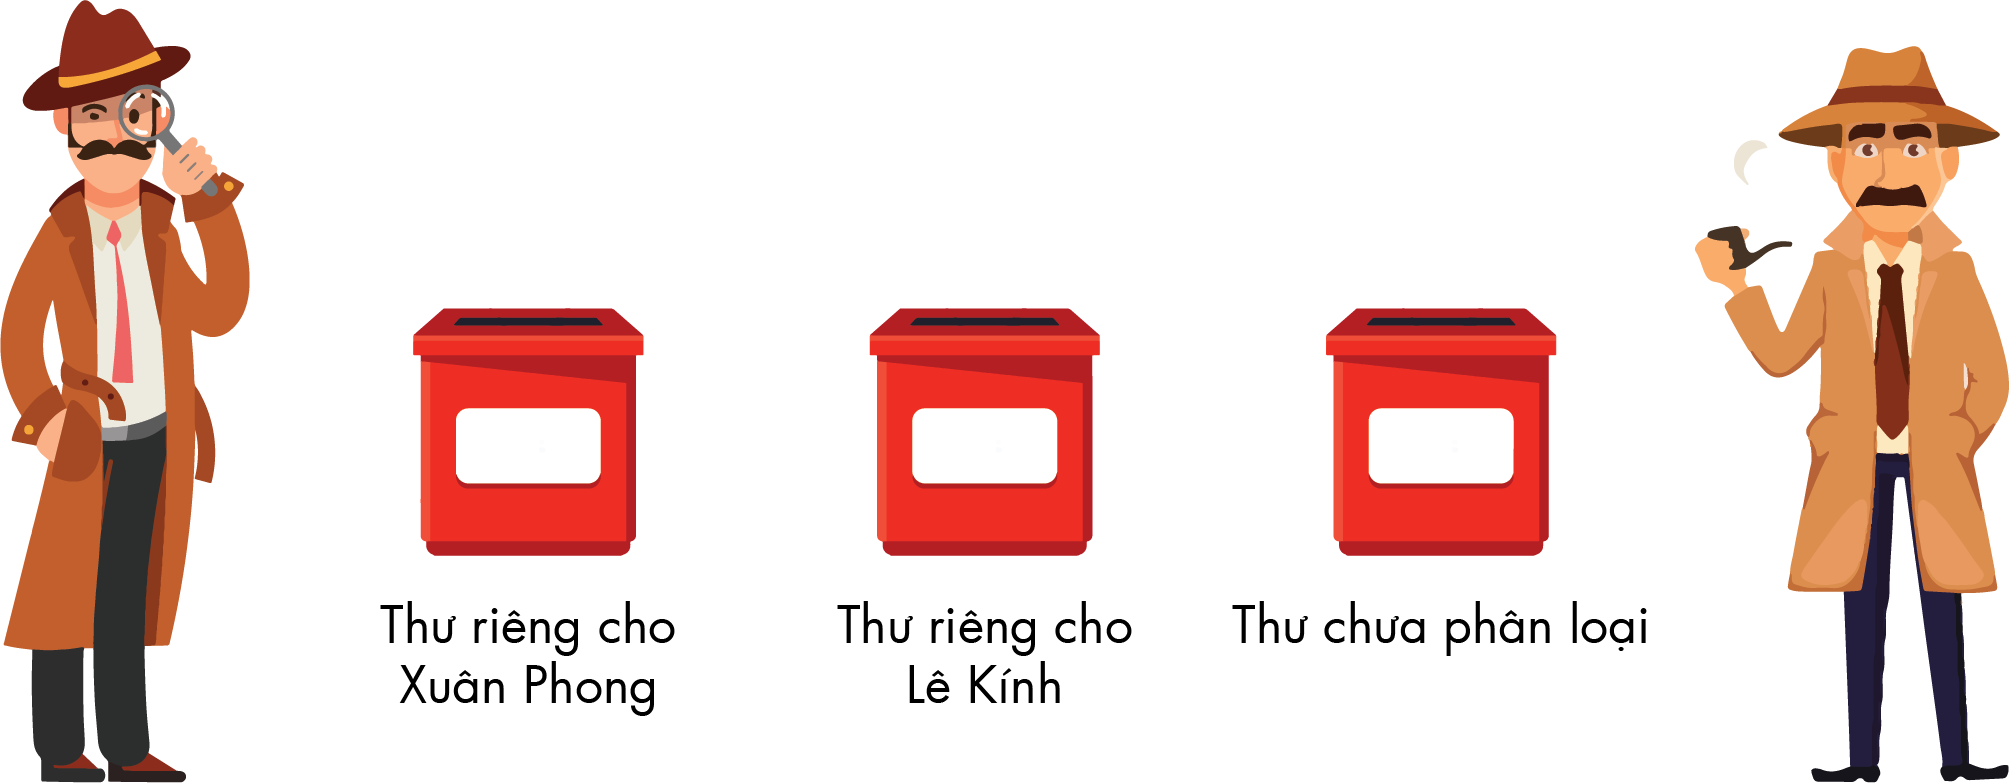
\includegraphics[width=1\linewidth]{5}
			\vspace*{-15pt}
		\end{figure}
	Chiều đã muộn, ngày cuối năm bận rộn, mà không ai trong văn phòng của Pi muốn về, tất cả vẫn say sưa nghe thanh tra Lê Kính kể truyện. Bất chợt, cửa phòng bật mở và Xuân Phong bước vào, rồi nhanh chóng cùng Lê Kính rời đi. Chắc là có một vụ án gấp cần hai thần tượng của chúng ta ra tay giải quyết. Mặc dù phải đi gấp nhưng thanh tra Lê Kính vẫn kịp nhắn: thám tử Xuân Phong đang chuẩn bị mở câu lạc bộ Thám tử nhí, 10 bạn đầu tiên tìm được nhiều câu trả lời đúng nhất cho những câu chuyện trên thì sẽ được tham gia vào câu lạc bộ này. Tất nhiên là có ưu tiên cho các độc giả của Pi. Các bạn nhỏ ơi, tết này vừa ăn vừa chơi, vừa tìm lời giải cho những tình huống của Xuân Phong để được là thành viên của câu lạc bộ Thám tử nhí nhé.
	